\subsection{Policy Setting: How are Local Roads Funded in Ohio?}

The policy setting is useful because renewal levies connect a concrete household tax bill to a dedicated local maintenance service. Voters are not deciding whether to start an unusually large capital project; they are deciding whether to continue an existing revenue stream for the upkeep of roads already in place. This section describes the institutional details needed to interpret those votes and the data used to measure their consequences.

Roads in Ohio are funded through a combination of federal, state, and local sources. A significant portion of road funding provided by federal and state governments comes from gas taxes, which are currently set at $\$0.18$ per gallon for the federal tax and $\$0.38$ per gallon for the Ohio state tax. Additional sources for these two levels of government include vehicle registration fees, license plate fees, tolls, and driver's license fees. Funding for local governments largely comes from property taxes. Below, we provide an overview of road funding in Ohio from national, state, and local sources.

{\bf Federal Funding.} U.S. Department of Transportation provides funding for road infrastructure through the Federal Highway Administration (FHWA). The FHWA provides funding for the construction, maintenance, and operation of highways, bridges, and tunnels. The federal government provides funding for road infrastructure through the Highway Trust Fund (HTF), which is funded by the federal gas tax. The HTF is divided into two accounts: the Highway Account and the Mass Transit Account. The Highway Account is used to fund highway construction and maintenance, while the Mass Transit Account is used to fund public transportation projects. The federal government also provides funding for road infrastructure through the Surface Transportation Block Grant Program or Bipartisan Infrastructure Law \citep{USDOT_BIL_Ohio}, which provides funding for road projects that are not eligible for funding through the HTF. Nevertheless, federal government funding for road infrastructure is generally limited, as in 2022, about 4/5$^\text{th}$ of all funding came from state and local governments \citep{pgpf_htf_explained}.

{\bf State Funding.}
In Ohio, gas taxes, licensing fees and user fees account for $69\%$ of the state's road funding \citep{boesen2021}. The Ohio Department of Transportation is responsible for the allocation of state funds, which are used for both maintenance and new construction. However, about 70\% of funds goes to new highway construction, 2\% is given to local governments as grants and only 4\% of state funds are directed towards road maintenance \citep{odot2023}. The remaining funds are part of payroll and operating expenses and other miscellaneous expenses. Hence, most of the road maintenance funding for local, neighborhood-specific roads in Ohio comes from local governments.

{\bf Local Funding.} Local governments in Ohio fund roads mainly through property taxes, although the extent of this funding varies across different localities. These municipalities have the authority to levy property taxes specifically for road maintenance, providing a crucial source of funding for the upkeep of local infrastructure. For instance, as per our correspondence with Beavercreek Township, 61\% of its road funds come from property taxes, and only 8\% from gas taxes. Moreover, 77\% of funding for roads in Beavercreek Township is provided by the local government and 11\% of the overall local government budget is allocated to roadway maintenance \citep{schroeder2025}. Local roads are primarily funded by local governments in Ohio and road maintenance funding is a significant part of the local government's budget.


\subsection{Local Taxation in Ohio}

{\bf Background.} Ohio consists of 88 counties, each covering about 464 square miles\footnote{This is roughly 1,200 square kilometers.}. Each county was historically divided into about 15 equally-sized townships, which do not cross county lines. Citizens can petition to incorporate as a village, which has a different type of government structure than a township and the ability to levy both income and property taxes, whereas townships may only levy property taxes. When a village exceeds 5,000 population in Ohio, it is reclassified as a city. Villages and cities may cross township and county lines, dissolve, or annex parts of contiguous townships. Villages, cities and townships, which we call “cities” for brevity, are the most local governmental unit in Ohio. Each local government covers about 18.2 miles$^2$ (47.1 km$^2$) on average. The Ohio Revised Code (ORC) separates property taxes into unvoted and voted levies. Local governments can levy unvoted property taxes up to 1\% of the assessed value of property without voter approval. Beyond this limit, local governments must seek voter approval through tax levies. These levies can be for new taxes or for the renewal of existing taxes, and can be earmarked for specific purposes such as building a new school, funding police and fire departments, or maintaining local roads. We focus on renewal levies slated for road maintenance. Our data on renewal road tax levies include 3,184 referendums and cover 617 local governments in Ohio.

% Ohio has 3,939 local governments in total as of 2022 \citep{stlouisfed2024local}.  

The type of tax levy we study is for the renewal of road tax levies. Most of the renewal taxes we consider have stated purposes of ``road and bridges repair'', ``road repair'', ``street fund'', and ``street improvements'', although there are less common stated purposes like ``repair and maintenance of streets and sewers system'' and ``resurfacing and rehabilitation of city streets''\footnote{These purposes are as per the financial reports of the local governments.}.  The construction of new roads and bridges, in contrast, would be funded with a tax levy for additional money, not a renewal tax; and it would likely be funded by a bond levy lasting 20 or 30 years.  
% We eliminate from our dataset stated purposes that might suggest new road construction like a 30-year 1.9-mill new tax in Moscow Village for ``permanent improvements'' and 0.5-mill new tax for 20 years in Shawnee Hills Village for ``general construction and road and bridges repair''. 
Our dataset includes tax levies such as a 2-mill, 5-year renewal in Adams Township (Champaign County) in 1995; a 3-mill, 5-year renewal in Lore City Village in 2016; and a 2.5-mill, 5-year renewal in Pataskala City in 2007.

{\bf Renewal levies.} Levies that had originally passed typically expire, and the most common duration to collect a levy is five years, representing about 90\% of the road tax levies in our sample. When a levy expires, voters have the option to renew it or let it lapse. If a tax levy is renewed, taxes and funding from that revenue stream continues. If 50\% or fewer votes approve the levy, it fails.  When a tax levy for additional funding fails, there is no increase in funding, but existing funding from other tax levies continues as normal.  When a renewal tax levy fails, funding from that tax levy stops. 99\% of the road tax levies in our sample are property taxes\footnote{The remaining 1\% are income taxes.}.

Most RD studies that use voting data to look at the impact of funding changes examine new tax levies for additional funding.  \cite{cellini2010value} observes that votes for additional tax money may not be statistically independent; a vote may be proposed until it passes.  We minimize this source of endogeneity of new votes by only considering renewal votes \citep{brasington2017school}.  While a government may choose when to put a vote for additional funding on the ballot and keep proposing the new tax until it is passed, when a vote passes, it has an expiration date.  So if a road tax levy for additional funding passes in 2007 to last five years, in 2012 voters will have the chance to renew or reject the tax.  The timing of the vote in 2012 is not endogenous, having been set in 2007.  If voters renew it in 2012, it will be up for renewal again in 2017. The exogeneity of the timing of a renewal tax levy contrasts with the timing of new taxes for additional money as explained by \cite{cellini2010value} because local governments can endogenously choose the timing of a new tax levy to coincide with positive economic conditions or positive sentiment toward government action, making an election more likely to pass.

{\bf Spending impact of failing to renew a levy.} When a renewal tax levy fails, the local government loses the funding from that tax levy. The local government may still have tax levies for other purposes in effect, but the road tax levy that failed to renew is no longer collected. We determine the dollar amount in consideration when a household is making a decision on whether to vote for or against a renewal road tax levy, and we call it Average Road Tax per household, which is the tax amount that a household will pay if the levy is successfully renewed. Average Road Tax per household is computed following Equation \ref{eq:avg_road_tax_per_household}:

\begin{equation}
\text{Average Road Tax per household}_{it} = \text{millage rate}_{it} \times \text{Average Assessed value}_{it}
\label{eq:avg_road_tax_per_household}
\end{equation}

\noindent where $i$ is the city, $t$ is the year, and millage-rate\footnote{Millage-rate is property tax rate expressed in mills (tax per \$1,000 of assessed value).} is the predetermined millage amount set for the road tax levy. The Average Assessed value is 35\% of the average appraisal value\footnote{Assessment ratio of 35\%, as set by \cite{OhioRealPropertyTax}.}, which for our study equals the average sale price of houses in the city for that year. From this, we can also compute the average road tax per city by multiplying the average road tax per household with the number of households in the city.

Although we acknowledge a large variation in the appraisal value across cities and in millage rates across referendums, we find that the average road tax per household is \$76, and the average road tax per city is \$167,011 as shown in Table \ref{tab:levy_stats}. We do not observe any significant difference in the average road tax per household between cities that renew and cut road tax levies, which suggests the levies up for renewal are not systematically different between areas that renew and areas that fail to renew them. Whenever a renewal tax levy fails, the local government loses the funding from that tax levy, which is the average road tax per city. This loss in funding directly impacts local government's spending budget needed to maintain local roads in Ohio and accounts for 11\% of a local government's budget for road maintenance\footnote{For townships within our effective bandwidth, we use the average expenditure by the public works department as our base, which is \$1,528,404 as per their audited financial reports. All local roads in such municipalities are funded via this department. Average loss in maintenance spending for areas that cut their renewal levy is \$163,547, thus giving us $11\% = \frac{163,547}{1,528,404} \times 100$ }.

\begin{table}[H]
    \centering
    \caption{Spending impact of failing to renew a Road Tax Levy}
    \label{tab:levy_stats}
    \begin{threeparttable}
    \begin{tabular}{p{5cm}ccc}
    \hline\hline
    & \textbf{Aggregate} & \textbf{Renewed} & \textbf{Cut} \\
    \hline
    \textbf{Panel A: road tax per household} \\
    Mean & 76 & 75 & 79 \\
       & (55) & (53) & (62) \\
    \hline
    \textbf{Panel B: road tax per city} \\
    Mean & 167,011 & 167,648 & 163,547 \\
       & (340,268) & (340,628) & (338,671) \\
    \hline\hline
    \end{tabular}
    \begin{tablenotes}[flushleft]
      \footnotesize
      \item \textit{Notes:} 
      This table presents descriptive statistics for two measures of the money collected via road tax levies. 
      \textbf{Panel A} reports the mean and standard deviation (SD) of the road tax per household per year. 
      \textbf{Panel B} reports the mean and SD of the total road tax collected per city. 
      “Aggregate” denotes the full sample, while “Renewed” and “Cut” refer to levies that were renewed and failed to renew respectively.
      All monetary values are in constant 2010 U.S. dollars and rounded to the nearest integer.
    \end{tablenotes}
    \end{threeparttable}
\end{table}

\subsection{Running Variable}

The running variable plays a critical role in RD, which in this study represents the proportion of votes against the renewal of a road tax levy. A vote share of 50\% or more against the renewal road tax levy means the levy fails and the tax will no longer be collected, resulting in a stoppage of road funding via that particular tax levy. There are 3,184 referendum results in our sample, 83\% of which renew the tax, and 17\% of which cut taxes and road maintenance. The Great Financial Crisis falls in the middle of our dataset, so readers might wonder if voting behavior was affected, but we find vote share the same to two decimal points during and outside the years 2008-2009. Our key identification assumption is that the election results are not predetermined and vote share is not precisely manipulated to fall just above or below the cutoff. This assumption allows us to exploit the randomization around the cutoff and provides the variation needed to identify the causal effect of cutting road tax. We test this assumption using a density test detailed below and covariate balance tests (see Appendix \ref{sec:appxb}).

{\bf Density test.} A classic RD assumption states that agents cannot precisely manipulate the running variable to fall just above or below the cutoff. In our context, it means that the election results are not determined prior to when the ballot takes place. In other words, no individuals, organizations, higher levels of government, foreign governments, or the firm that programs the voting machines are dictating the precise vote share for the renewal road tax levy referendums raised by a city. The standard way to test this assumption is to perform a density test like that of \cite{cattaneo2020simple}, which is based on the idea that manipulation of elections might cause a clustering of votes just to one side of the cutoff, with a pronounced drop-off on the other side of the cutoff. The $p$-value of this density test is 0.98. A histogram of vote share is shown in Figure \ref{fig:running_var_hist} that graphically illustrates the lack of abrupt change in density.

\begin{figure}[ht]
    \centering
    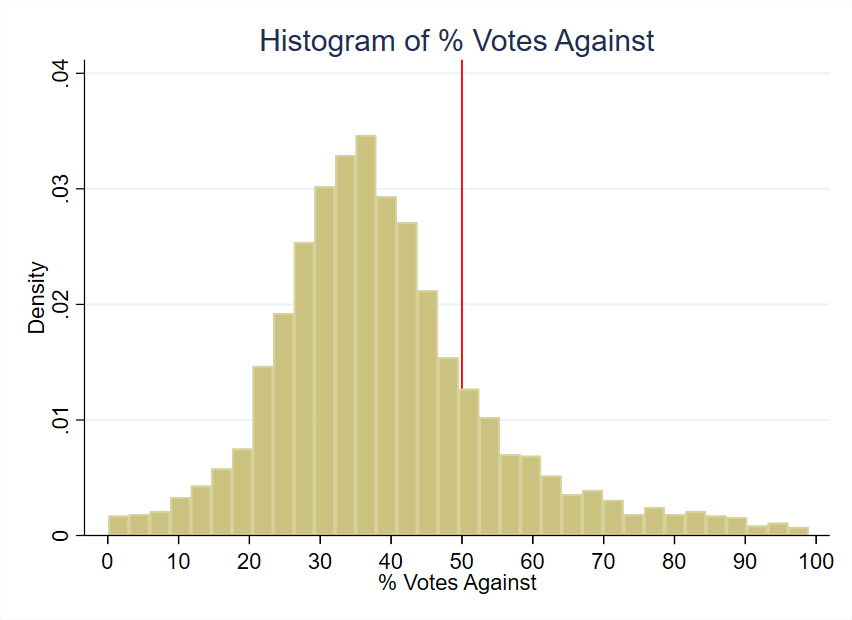
\includegraphics[width=\textwidth,keepaspectratio]{images/votes_pct_against_histogram.png}
    \caption{Histogram of Running Variable}
    \label{fig:running_var_hist}
\end{figure}

Although Table \ref{tab:variable_means_sd} shows covariate balance between sets of cities that pass and fail to renew road tax levies, covariate values could still jump from one side of the cutoff to another. A drop in education levels, for example, could cause a drop in house prices that might coincide with a change in treatment, so that what might look like a treatment effect from cutting taxes and spending might in fact be caused by lower education levels. Graphs that suggest covariate smoothness around the cutoff are found in Appendix \ref{sec:appxb}. A formal way to assess covariate smoothness is to use each covariate as an outcome variable in a regression of the running variable and the treatment effect dummy. When we do so, the $p$-value of the treatment effect dummy varies from 0.234 to 0.981, as shown in Table \ref{tab:covariate_discontinuity}, indicating no statistically significant jump in covariate values. 

\subsection{Outcome Variable: Median House Price}

Our house price data comes from a CoreLogic® dataset of actual sales transaction prices in Ohio from 1995 through 2021 containing over 7 million observations. The dependent variable, \textit{Median House Price}, reflects the median sale price of houses within a specific city and year. For example, for the houses sold in Delaware Township during the year 2002, the median sale price was \$205,041. We take precaution to only include arm’s-length transactions, and we restrict our attention to single-family residential structures for comparability.  The overall sample mean for the 10-year period from the time of votes considered in this study is \$166,082 in constant 2010 dollars with a standard deviation of \$372,135 which suggests the presence of outliers. Although our use of median sale price addresses outliers, one of our robustness checks drops 1\% tails and re-estimates the treatment effects (Figure \ref{fig:tes_g_w}).  
% The mean for this winsorized sample is \$150,375 in constant 2010 dollars with a standard deviation of \$116,020. 

\begin{figure}[ht]
    \centering
    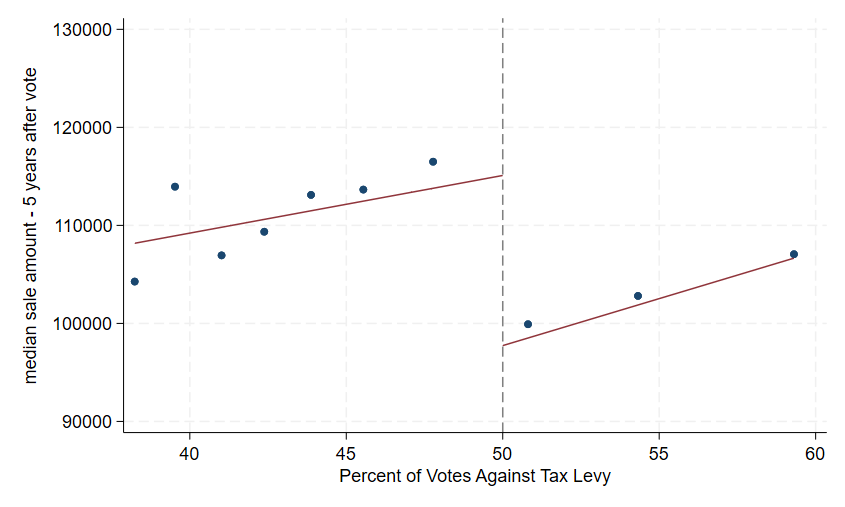
\includegraphics[width=0.8\textwidth,keepaspectratio]{images/rd_plot_year_5_after_vote.png}
    \caption{Median Sale Price of Houses: 5 years after vote}
    \label{fig:hp_year5_after}
\end{figure}

Figure \ref{fig:hp_year5_after} shows house prices from five years after the vote graphed alongside the percent of votes against the tax levy\footnote{after deflating to 2010 U.S. dollars}. The points represent the mean house price for the 10 representative bins of vote shares for the average effective bandwidth around the cutoff of 50\%. This visual pattern indicates a discrete jump in house prices at the 50\% threshold, implying that tax levy failures lead to reduced property values.

% We also sample financial audits of cities in our sample whose renewal tax levies fail.  

\subsection{Road Quality} \label{sec:road_quality}

Roads in Ohio last 15-20 years and deteriorate faster with poor drainage, utility cuts to the road, and snowplow damage \citep{hudson2020faq}. 
% The maintenance that occurs is more often reactive like filling potholes rather than proactive like resurfacing. This reactive approach to maintenance raises concerns about the long-term quality of local roads, especially when funding from local roads is reduced or eliminated. 
To understand the effect of cutting local road taxes on road quality, we fine-tune an AI vision model on satellite imagery data from \cite{brewer2021}. Following the seminal work on text-based Transformers in Natural Language Processing (NLP) by \cite{vaswani2017attention}, vision transformers (ViTs) were introduced by Google Brain's team and are part of a recent class of deep learning models that have shown to outperform classic Convolutional Neural Networks (CNNs) on image classification tasks \citep{dosovitskiy2020image}. Nevertheless, a more recent class of vision models learns from ViTs and uses CNNs to achieve high accuracy on image classification tasks \citep{woo2023convnext}. We use one such model to classify road quality from satellite images\footnote{see the Appendix, Section~\ref{sec:appx_finetune} for details.}. Below, we outline the steps we take to assess road quality.


% We use the vision model to classify road images into three categories: good, average, and poor. We then use the classification results to assess the quality of roads in different neighborhoods in Ohio. We collect road images for areas that were within the average effective RD bandwidth provided in Table \ref{tab:median_sale_amount} and ensure that we have pre and post referendum images for both, the treatment and control groups. This allows us to construct a novel database of road images and assess the impact of cutting local road tax on road quality.

{\bf Satellite Images for fine-tuning.} Fine-tuning a vision model involves taking a pretrained model and adapting it for a specific image-classification task. 
% We fine-tune OpenAI's gpt-4o, a pretrained multi-modal Large Language Model (LLM) with over 200 billion parameters that has been shown to outperform various other models and benchmarks \citep{achiam2023gpt}. 
In order to ensure appropriate fine-tuning and enable our vision model to accurately predict road quality, we need large-scale road-image data. We use the road-image dataset of \cite{brewer2021} which consists of 53,677 labeled satellite images of roads in different conditions, and a classification representing quality of each road: 0 (poor), 1 (decent) and 2 (high). We divide the data into training, validation and test datasets, and use 70\% of the data for training, 15\% for validation and 15\% for testing. 
For a detailed analysis of the road-image dataset, see the Appendix, Section~\ref{sec:appx_finetune}.
% Using Hugging Face, we set up a training seed, convert the images into their corresponding base64 encoding, and fine-tune the model on the road-image dataset for 10 epochs with a batch size of 9 and a learning rate multiplier of 2. 
In section \ref{sec:road_quality_decline}, we present the results from our fine-tuned model, when applied to roads in areas with close elections within the effective bandwidth. 
% For full details on the modeling methodology, fine-tuning results and robustness tests, see \cite{2025predicting}.

{\bf Ohio Roads Imagery.} While the fine-tuning of our vision image-classification model uses images from \cite{brewer2021}, our Ohio application uses road-centered aerial imagery collected from public imagery sources. We first use Google Earth Engine to collect images from the National Agriculture Imagery Program (NAIP), which provides repeated high-resolution aerial imagery for Ohio over much of our study period\footnote{We considered using Google Earth Pro for satellite images but found these images too sparse to form a panel dataset for our study.}. To make sure the imagery corresponds to actual roads, we begin with TIGER road geometries that are spatially joined to county subdivisions, sample points along road line segments in each subdivision, and download image chips centered on those road points\footnote{An image chip is a small cropped tile from a larger aerial image centered on the road location used for prediction.}. Each chip covers a fixed ground window around the sampled road location, and the image manifest records the county-subdivision identifier, road name, image year, latitude, longitude, and file name. This procedure yields a panel-like set of road images across subdivisions and years\footnote{We also construct a companion set of images from the Ohio Statewide Imagery Program (OSIP3) using the same road-point sampling strategy. OSIP3 provides sharper imagery for later years, and we use it to check and supplement coverage in supporting diagnostics. However, because OSIP3 begins only after 2017, the main road-quality estimates in Table \ref{tab:roadquality_estimates} report NAIP-based Road Quality Rating and Road Quality Score outcomes so that the units remain directly interpretable across post-election windows. The pooled NAIP-OSIP3 standardized estimates are used only in supporting diagnostics.}. In the empirical analysis, predicted road quality is aggregated within pre-election and post-election windows around each renewal election, election-year imagery is omitted, and each window is censored at adjacent renewal elections so the same subdivision-year is not reused across levy cycles.

% Figure \ref{fig:road_quality_examples} presents two examples of road satellite images for Ohio, one from a road classified as high and the other as poor quality.
% \begin{figure}[ht]
%     \centering
%     \begin{minipage}{0.59\textwidth}
%         \centering
%         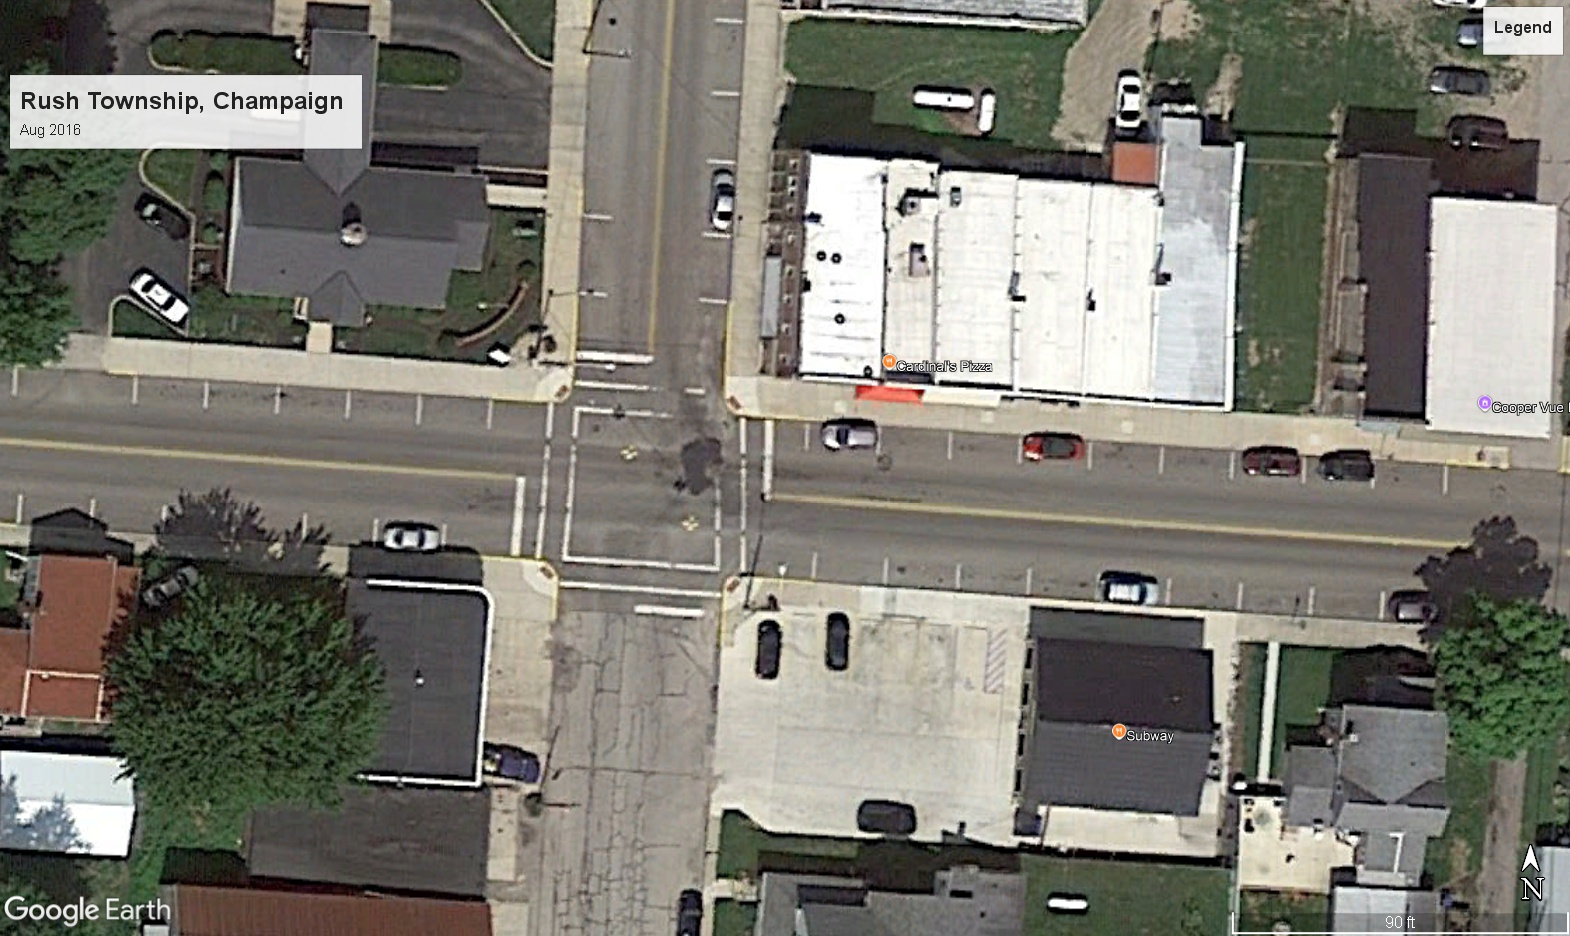
\includegraphics[width=\textwidth]{images/rush_twp_champaign_aug16.jpg}
%         \caption*{(A) A {\bf \underline{Poor}} Quality Road}
%     \end{minipage} 
%     \hspace{0.5in}
%     \begin{minipage}{0.59\textwidth}
%         \centering
%         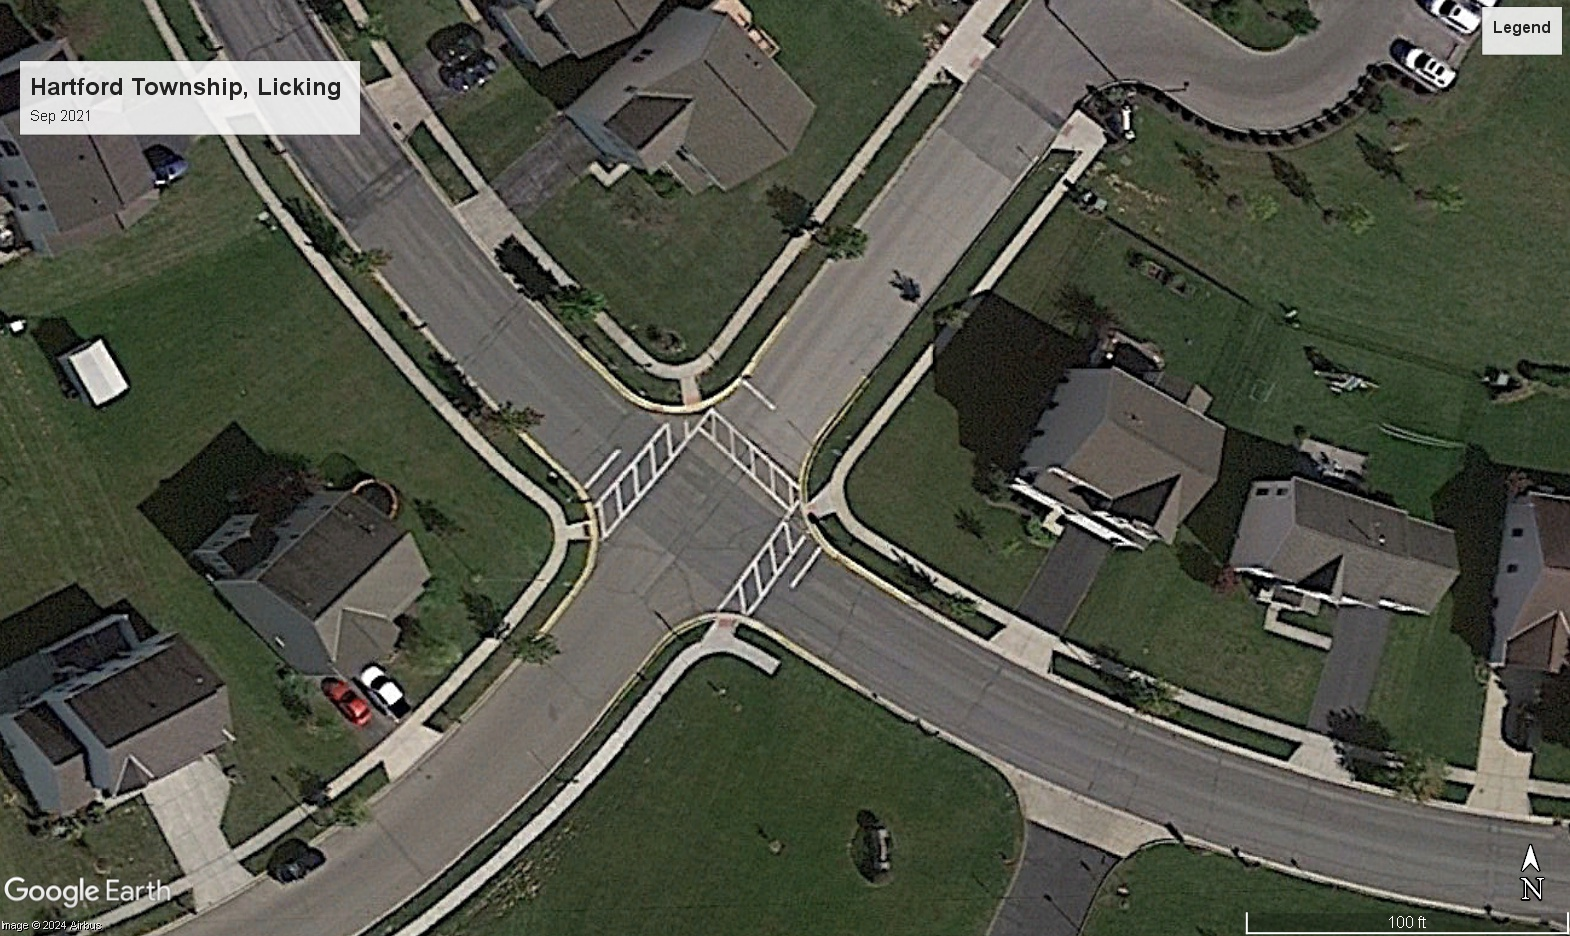
\includegraphics[width=\textwidth]{images/hartford_twp_licking_sep21.jpg}
%         \caption*{(B) A {\bf \underline{High}} Quality Road}
%     \end{minipage}
%     \caption{Road Quality Satellite images for Ohio}
%     \label{fig:road_quality_examples}
% \end{figure} 

{\bf Road Quality Metrics.}  For road quality analysis, we use two metrics derived from our fine-tuned vision model: the Road Quality Rating (RQR) and the Road Quality Score (RQS). 

\textit{Road Quality Rating.} Our fine-tuned vision model classifies each road image into one of three categories: 0 (poor), 1 (average), or 2 (high). This rating is based on visual cues such as pavement quality, visible cracks, patchwork, and overall surface condition, as learned by the vision model from the labeled training data. For each image, the model outputs both the predicted class and a confidence score, which reflects the model's certainty in its prediction. These ratings provide a standardized, objective measure of road quality across locations and time periods, enabling us to compare changes in road conditions before and after tax levy referendums for both treated and control groups.

\textit{Road Quality Score.} Even though our original model output is a road quality rating\footnote{This is a direct result of our training data from \cite{brewer2021} which uses the discrete 0 (low), 1 (medium), 2 (high) road-quality metric.}, we also convert the discrete model output to a continuous Road Quality Score (RQS). This conversion uses two variables: the predicted road quality rating and the confidence score\footnote{During the prediction process, we asked the fine-tuned vision model its confidence in the prediction i.e. the probability of the prediction being correct, a number between 0 and 1.}. The formula for this conversion is as follows:

\begin{equation}
\text{RQS} = 1 + b
\begin{cases}
1 - w\hat{c}, & \hat{r}=0,\\
\hat{r} + w\hat{c}, & \hat{r}\in\{1,2\}.
\end{cases}
\label{eq:rqs_formula} 
\end{equation}
 
\noindent 
where $\hat{r}$ is the predicted road quality rating and $\hat{c}$ is the confidence score. The parameter b determines the size of each rating bin, and $w$ determines the weight of the confidence score which determines the sensitivity within the predicted class\footnote{We set $b$ to $\frac{99}{3}$ to give the three rating bins equal width and set $w$ to 0.5.}. Higher confidence in a poor classification lowers the score, while higher confidence in average or high classifications raises it\footnote{This allows the model to adjust the score based on its confidence in the prediction, providing a more nuanced measure of road quality. Under this specification, RQS ranges from 18.2 to 83.5, with larger values indicating higher road quality.}. We use this RQS metric in our analysis to assess the impact of cutting local road taxes on road quality.

Next, we share a summary of means and standard deviations of the predicted road quality rating and road quality score for the treatment and control groups, before and after the referendum. 

\begin{table}[H]
    \centering
    \caption{Predicted Road Quality by Treatment Status and Period}
    \label{tab:road_quality_panel}
    \begin{threeparttable}
    \begin{minipage}{\linewidth}
    \centering
    \setlength{\tabcolsep}{5pt}
    \begin{tabular}{lccccc}
        \toprule
        & \multicolumn{2}{c}{\textbf{Global}} & \multicolumn{3}{c}{\textbf{Effective}} \\
        \cmidrule(lr){2-3} \cmidrule(lr){4-6}
        & Control & Treated & Control & Treated & Difference \\
        & (Renewed) & (Failed) & (Renewed) & (Failed) & (Treated$-$Control) \\
        \midrule
        \multicolumn{6}{l}{\textbf{Panel A: Road Quality Rating (0, 1, 2)}} \\
        Pre-Election ($t\!-\!3$ to $t\!-\!1$)  & 1.49 & 1.55 & 1.56 & 1.66 & 0.10 \\
                       & (0.24) & (0.19) & (0.07) & (0.06) & (0.10) \\
        Post-Election ($t\!+\!3$ to $t\!+\!5$) & 1.55 & 1.65 & 1.72 & 1.44 & -0.28$^{***}$ \\
                       & (0.23) & (0.18) & (0.05) & (0.07) & (0.07) \\
        \addlinespace
        \multicolumn{6}{l}{\textbf{Panel B: Road Quality Score (RQS)}} \\
        Pre-Election ($t\!-\!3$ to $t\!-\!1$)  & 61.4 & 63.4 & 64.1 & 66.8 & 2.7 \\
                       & (8.2) & (6.9) & (2.2) & (2.3) & (3.6) \\
        Post-Election ($t\!+\!3$ to $t\!+\!5$) & 63.1 & 66.6 & 69.0 & 59.2 & -9.8$^{***}$ \\
                       & (7.9) & (6.5) & (1.8) & (2.7) & (2.6) \\
        \bottomrule
    \end{tabular}
    \vspace{0.5em}
    \begin{tablenotes}[flushleft]
        \footnotesize
        \item \textit{Notes:} The treated group comprises observations that failed to renew their road tax levies. The control group comprises those that renewed. The sample is the ConvNeXt V2 stacked-event NAIP road imagery sample with valid pre- and post-window imagery. Election-year imagery is omitted and windows are censored at adjacent renewal elections. \textit{Global} columns are unweighted descriptive means across all observations with standard deviations in parentheses, with no bandwidth restriction. \textit{Effective} columns are local-linear RD fits at the 50\% vote-against cutoff, using the MSE-optimal bandwidth of $h\approx4.4$--$4.7$ percentage points; these are fitted values at the cutoff with standard errors in parentheses, and the treated value is the control fit plus the RD estimate. 
        The pre-election rows are a placebo balance check and show no significant treated--control gap at the cutoff (RQR $p=0.33$, RQS $p=0.45$), consistent with comparability near the threshold.
        \item Significance: *** $p<0.01$, ** $p<0.05$, * $p<0.1$.
    \end{tablenotes}
    \end{minipage}
    \end{threeparttable}
\end{table}


Table \ref{tab:road_quality_panel} reports the Road Quality Rating (RQR) in Panel A and the Road Quality Score (RQS) in Panel B. The \textit{Global} columns are unadjusted means over the full sample. If we naively compare these raw averages, treated areas do not look worse than control in the post-election window, as treated RQR is 1.65 against 1.55 for control, and treated RQS is 66.6 against 63.1. However, selection into the treatment group may not be random, and thus these comparisons may be biased due to observable and unobservable confounders.
Because jurisdictions that fail and renew levies may differ systematically, these global comparisons are descriptive only and need not reflect the causal effect.

The \textit{Effective} columns in Table \ref{tab:road_quality_panel} report local-linear fits at the 50\% vote-share cutoff, the local comparison underlying our identification strategy. The treated and control fits show no statistically significant differences in the pre-election window. After the election, road quality in the treated group is lower than control group: RQR is 1.44 against 1.72, and RQS is 59.2 against 69.0. The \textit{Difference} column compares the treated and control fits, reporting the bias-corrected RD estimate at the cutoff.
Section \ref{sec:road_quality_decline} provides a detailed analysis of these findings.


% \begin{figure}[ht]
    % \centering
    % \begin{minipage}{0.59\textwidth}
    %     \centering
    %     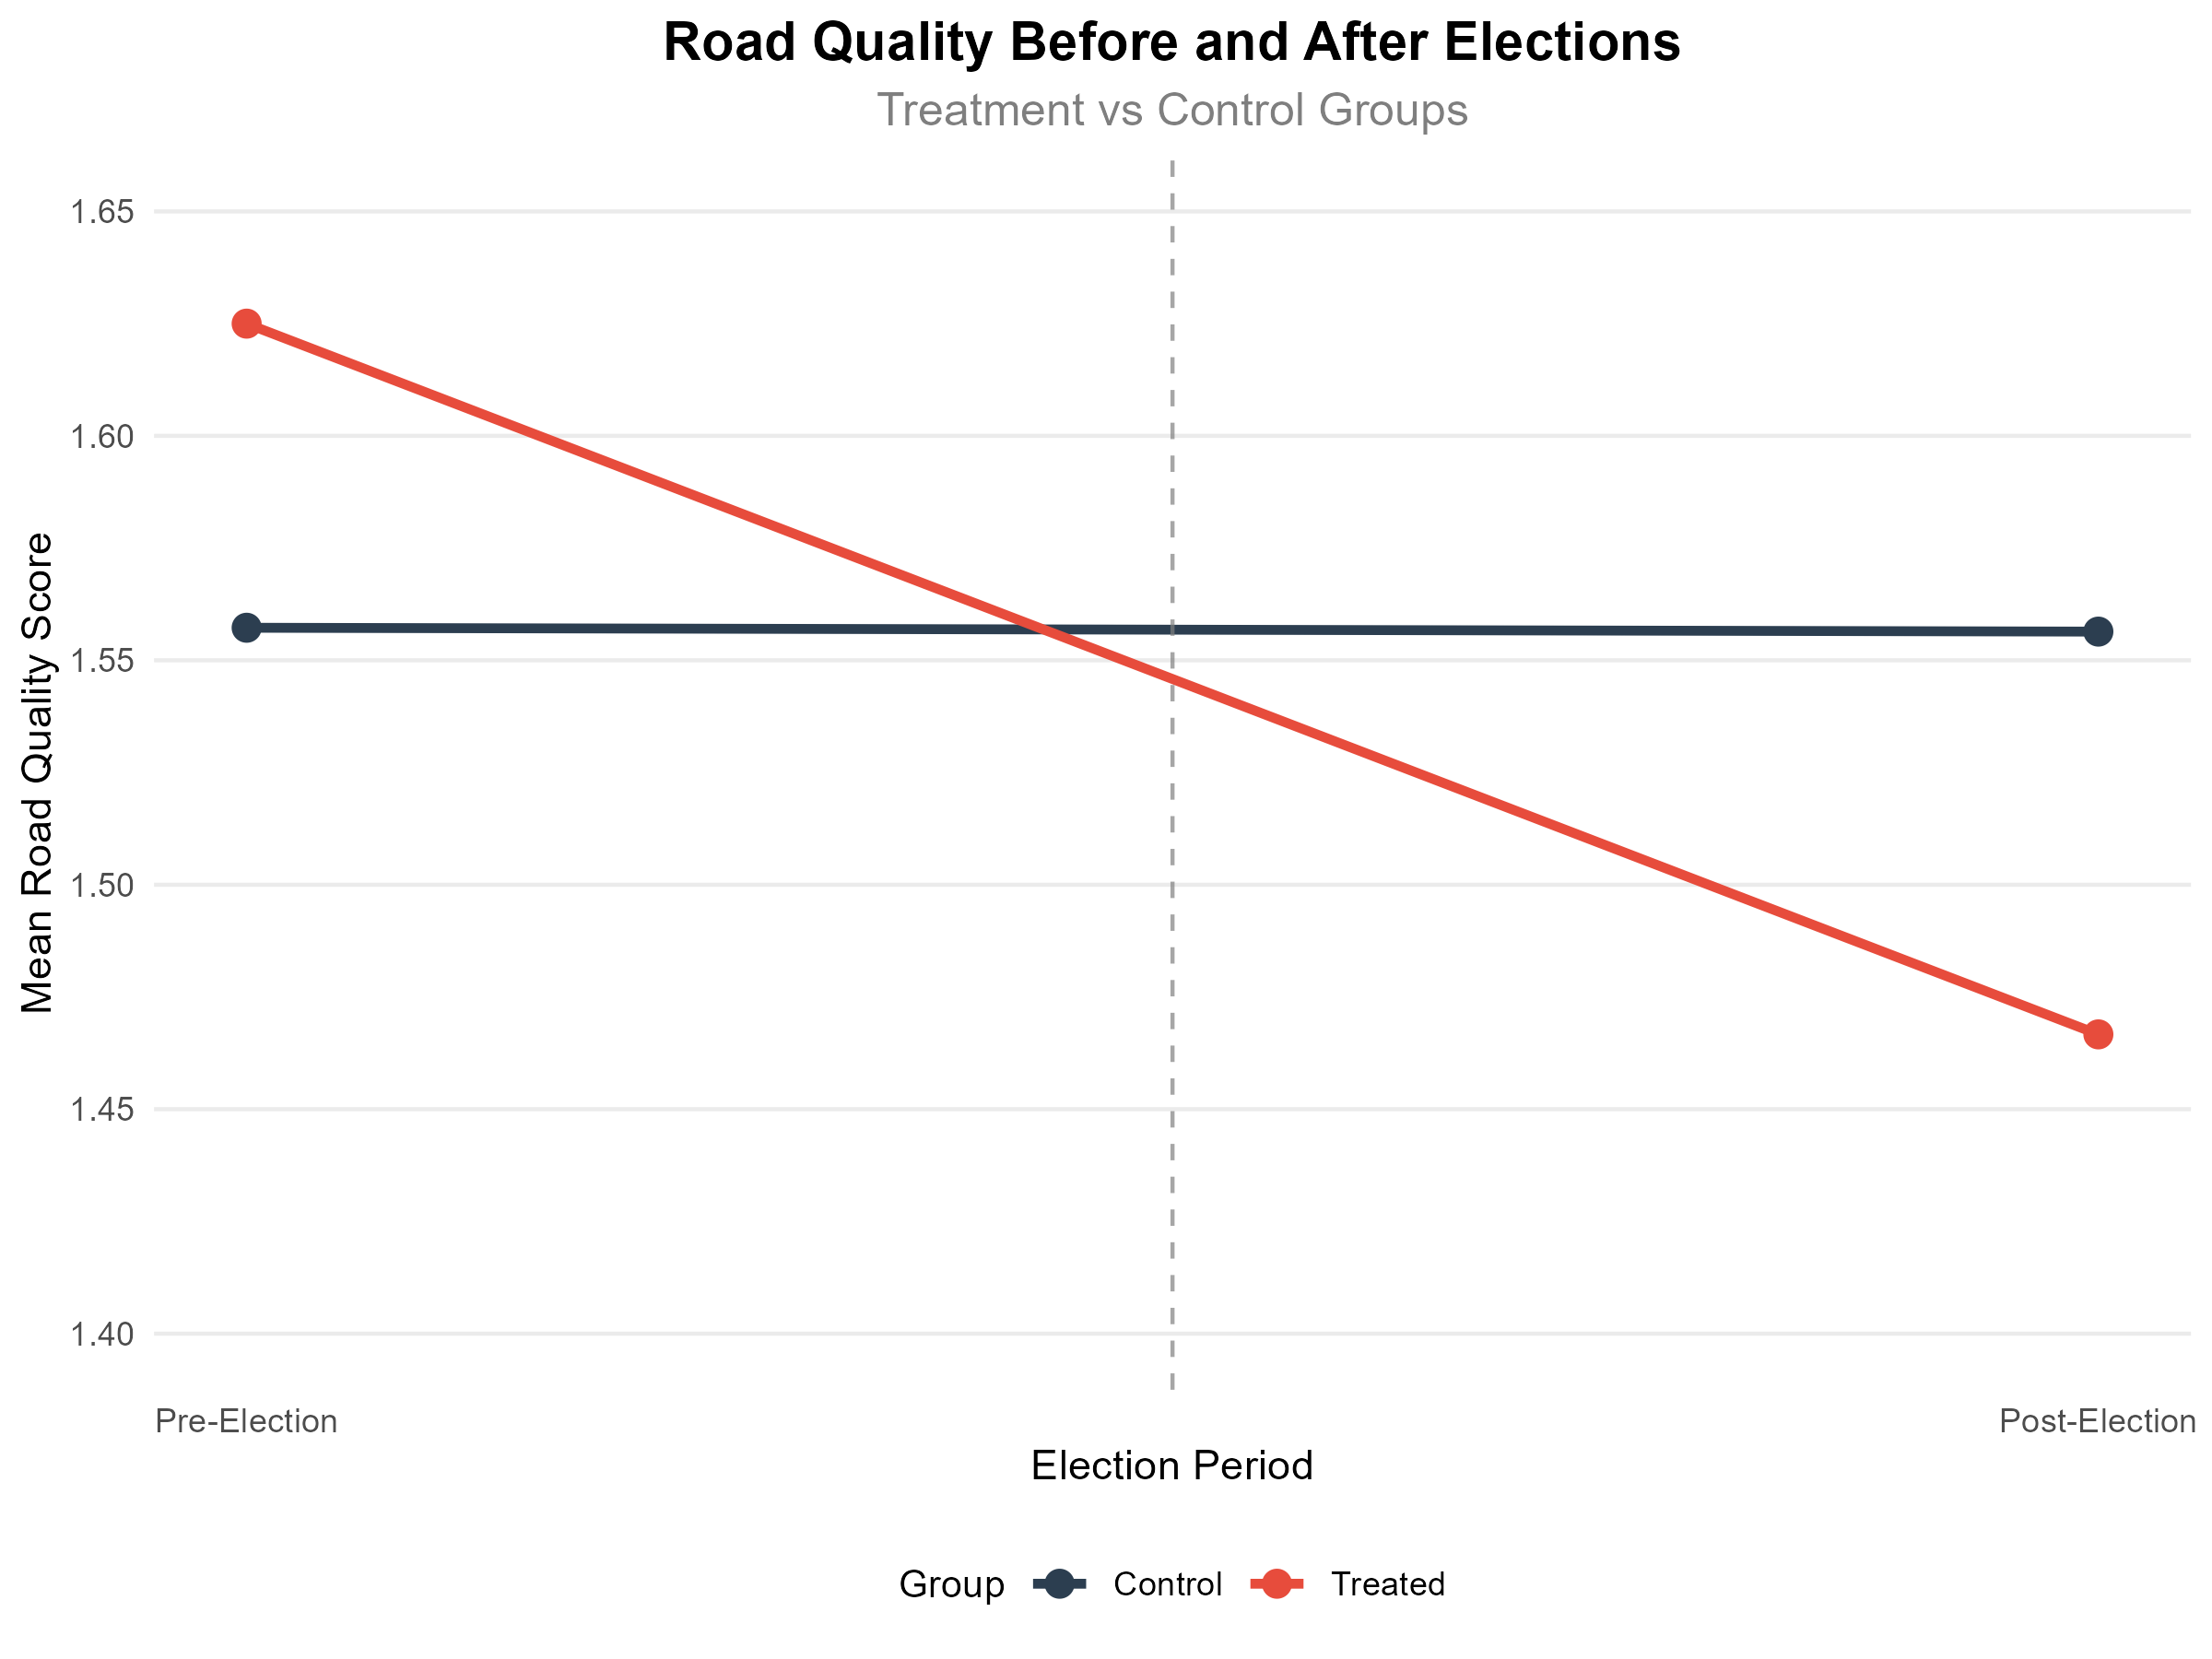
\includegraphics[width=\textwidth]{images/road_quality_lineplot.png}
    %     \caption*{(A) Before and after referendum}
    % \end{minipage} 
    % \hfill
    % \hspace{0.5in}
    % \begin{minipage}{0.59\textwidth}
    % \centering
    % 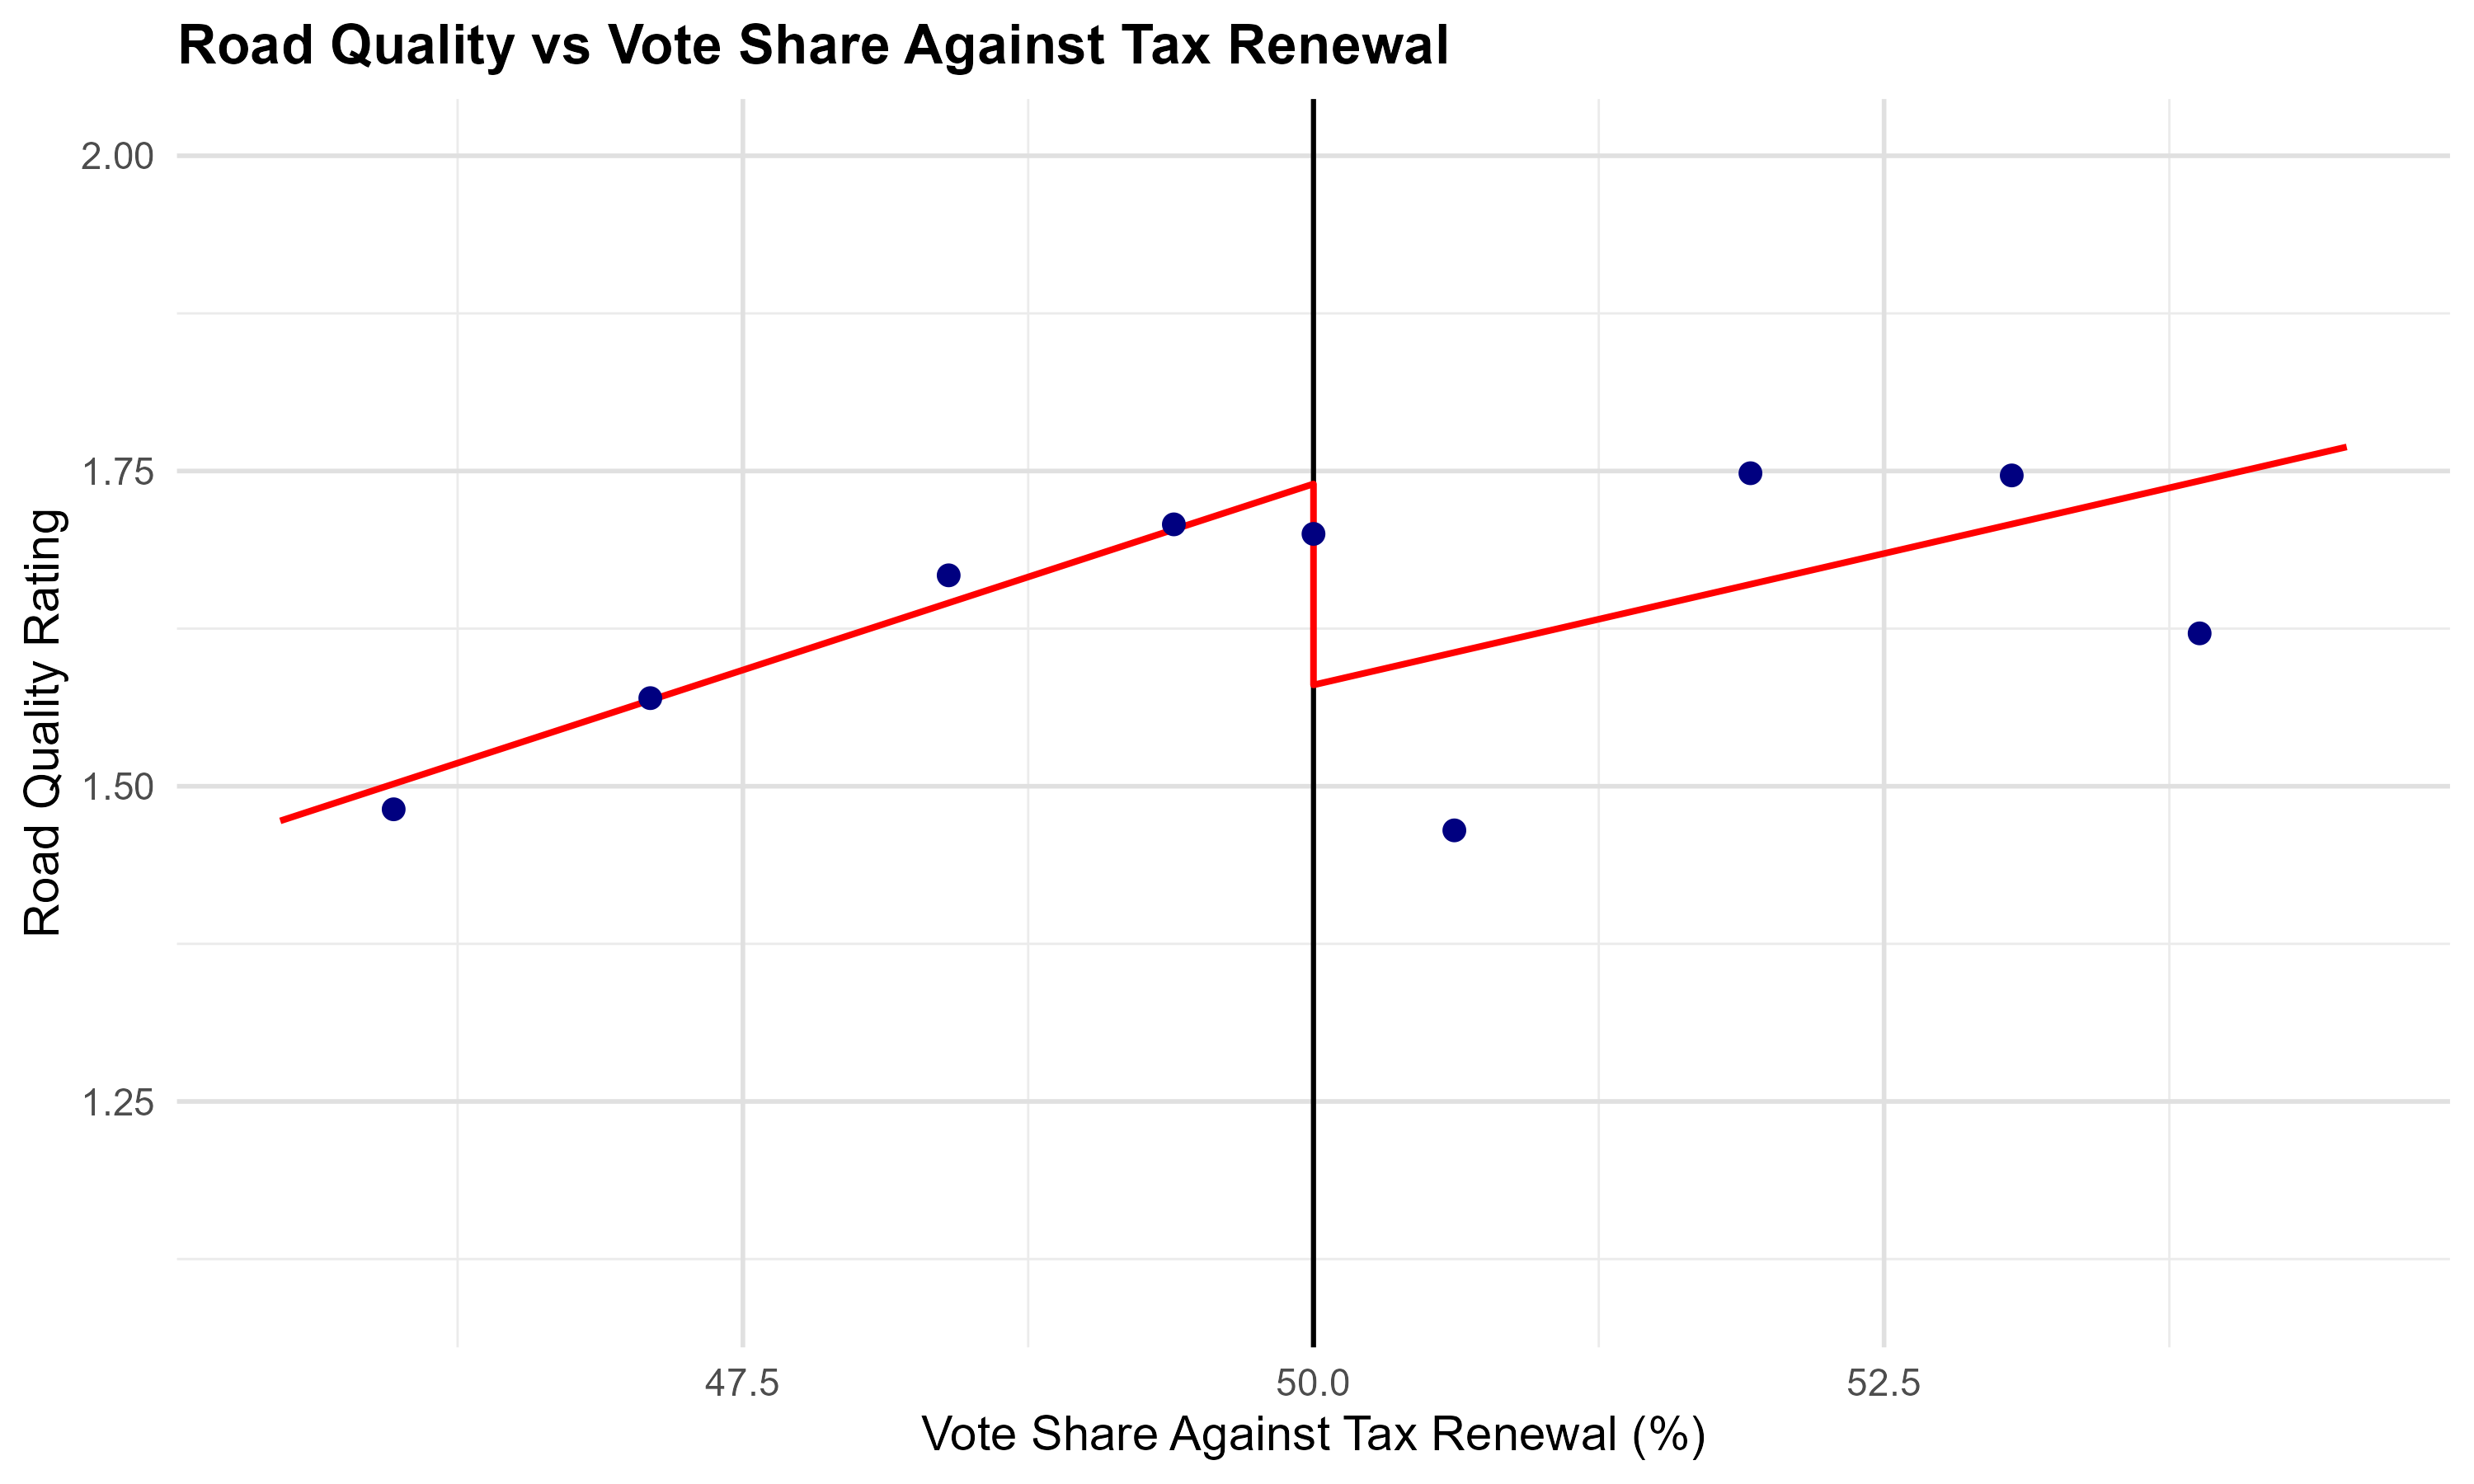
\includegraphics[width=\textwidth]{images/rd_plot_road_quality_naip_t2_t4.png}
    % \caption*{(B) Road Quality vs Vote Share Against Renewal (\%)}
    % \end{minipage}
%     \caption{NAIP Road Quality vs Vote Share Against Renewal (\%)}
%     \label{fig:combined}
% \end{figure}

% Figure \ref{fig:combined} Panel A graphically illustrates the difference in road quality rating before and after the referendum for both treated and control groups. The graph shows a clear decline in road quality rating for the treated group after the referendum, while the control group remains relatively stable. Panel B of 
% Figure \ref{fig:combined} shows the NAIP-based road quality rating in the $t+2$ to $t+4$ post-election window graphed alongside the percent of votes against the tax levy. The points represent the local average road quality rating for the representative bins of vote shares within the Table \ref{tab:roadquality_estimates} RQR bandwidth around the cutoff of 50\%. The graph reveals a discontinuity in road quality rating at the cutoff, which is the basis of our identification strategy, suggesting that the failure to renew a road tax levy has a negative impact on road quality. Section \ref{sec:road_quality_decline} provides a more detailed analysis of the impact of cutting road taxes on road quality, using the predictions from the model as the outcome variable, and employs regression discontinuity to estimate the effect of cutting road maintenance taxes on road quality.

% To address this, we implement a difference-in-differences (DiD) analysis in Section \ref{sec:road_quality_decline}, which controls for time-invariant factors and common shocks, allowing for a cleaner estimate of the effect of tax cuts on road quality.

\subsection{Covariates} 

Covariates can be useful in RD studies, although they are not necessary for the identification of treatment effects.  One use of covariates is to increase the precision of treatment effect estimates.  The other is to see if cities that barely pass and fail tax levies are similar to each other like the theory of RD says they should be. Table \ref{tab:variable_means_sd} shows covariate means for both the global sample of all votes in the data set as well as the local sample within a representative effective bandwidth of the 0.50 cutoff. The effective bandwidth displayed in Table \ref{tab:variable_means_sd} is the mean bandwidth for all the housing outcome regressions. The first columns for the global sample show similar values of characteristics between cities that renew and cut road taxes and spending, but it is the two rightmost columns that are critical for the credibility of the RD design.   

The data, captured at the time of the vote and as observed in Table \ref{tab:variable_means_sd}, shows minimal differences within the effective bandwidth: mean population differs by only 301, and median family income varies by \$436, measured in 2010 U.S. dollars. Other variables, including poverty rates, married household percentages, educational attainment, age distribution, and racial composition, show differences of two percentage points or less, bolstering the comparability of the treatment and control groups. This similarity supports interpreting post-election outcome differences near the cutoff as effects of the renewal decision rather than pre-existing differences\footnote{We also find similar covariate means for cities that have no road tax levies, which we explain in Section \ref{sec:robustness}}.

\begin{table}[H]
    \centering
    \caption{Variable Means \& Standard Deviation by Road Tax Levy Renewal Status}
    \label{tab:variable_means_sd}
    \begingroup
    \footnotesize
    \setstretch{1}
    \setlength{\tabcolsep}{3pt}
    \begin{tabular}{>{\raggedright\arraybackslash}p{3.4cm}ccccc}
    \hline
    Variable & \multicolumn{3}{c}{Global} & \multicolumn{2}{c}{Effective} \\
    \cmidrule(lr){2-4} \cmidrule(lr){5-6}
    & Full Sample & Renewed & Cut & Renewed (Control) & Cut (Treatment) \\
    \hline
    Population & 5,072 & 4,733 & 5,139 & 4,885 & 5,186 \\
                & (7,936) & (7,291) & (8,058) & (7,036) & (8,229) \\
    Poverty Rate & 0.11 & 0.11 & 0.11 & 0.10 & 0.11 \\
                    & (0.08) & (0.07) & (0.08) & (0.07) & (0.08) \\
    \% with Kids & 0.39 & 0.40 & 0.39 & 0.39 & 0.39 \\
                    & (0.08) & (0.08) & (0.08) & (0.07) & (0.08) \\
    \% Households with Children under 18 & 0.09 & 0.09 & 0.09 & 0.09 & 0.08 \\
                                            & (0.06) & (0.05) & (0.06) & (0.06) & (0.05) \\
    \% Less than High School Education & 0.16 & 0.18 & 0.15 & 0.18 & 0.16 \\
                                        & (0.11) & (0.12) & (0.11) & (0.12) & (0.10) \\
    \% Some College Education & 0.25 & 0.24 & 0.25 & 0.24 & 0.25 \\
                                & (0.06) & (0.06) & (0.06) & (0.07) & (0.06) \\
    \% Renters & 0.20 & 0.20 & 0.20 & 0.19 & 0.20 \\
                & (0.11) & (0.10) & (0.11) & (0.09) & (0.11) \\
    Unemployment Rate & 0.05 & 0.05 & 0.05 & 0.05 & 0.06 \\
                            & (0.04) & (0.03) & (0.04) & (0.03) & (0.04) \\
    \% White & 0.96 & 0.97 & 0.96 & 0.97 & 0.97 \\
                & (0.07) & (0.07) & (0.07) & (0.07) & (0.08) \\
    \% Black & 0.02 & 0.02 & 0.02 & 0.02 & 0.02 \\
                & (0.07) & (0.06) & (0.07) & (0.07) & (0.07) \\
    \% Married & 0.59 & 0.60 & 0.59 & 0.61 & 0.60 \\
                & (0.09) & (0.08) & (0.09) & (0.08) & (0.09) \\
    \% Separated & 0.01 & 0.01 & 0.01 & 0.01 & 0.01 \\
                    & (0.01) & (0.01) & (0.01) & (0.01) & (0.01) \\
    Income Heterogeneity Index & 0.10 & 0.09 & 0.10 & 0.09 & 0.09 \\
                                & (0.08) & (0.07) & (0.08) & (0.07) & (0.06) \\
    Median Family Income & 61,018 & 58,761 & 61,467 & 59,934 & 60,370 \\
                            & (17,649) & (13,915) & (18,270) & (13,655) & (15,713) \\
    \% Under 5 Years Old & 0.06 & 0.06 & 0.06 & 0.06 & 0.06 \\
                            & (0.02) & (0.02) & (0.02) & (0.02) & (0.02) \\
    \% Aged 5 to 17 & 0.20 & 0.21 & 0.20 & 0.20 & 0.20 \\
                    & (0.05) & (0.04) & (0.05) & (0.04) & (0.05) \\
    \% Aged 18 to 64 & 0.60 & 0.60 & 0.60 & 0.60 & 0.60 \\
                        & (0.05) & (0.05) & (0.05) & (0.04) & (0.05) \\
    \% Racial Minority & 0.04 & 0.03 & 0.04 & 0.03 & 0.03 \\
                        & (0.07) & (0.07) & (0.07) & (0.08) & (0.07) \\
    Number of Observations & 3,184 & 2,656 & 528 & 653 & 269 \\
    \hline
    \end{tabular}
    \begin{minipage}{0.95\textwidth}
        \vspace{0.2em}
        \footnotesize \textit{Notes:} Covariates are measured at the time of the vote. Standard deviations are in parentheses. ``Global'' refers to the full referendum sample with no bandwidth restriction. ``Effective'' refers to observations within the mean effective optimal bandwidth from the house price regressions in Table \ref{tab:median_sale_amount}. Renewed jurisdictions are the control group. Jurisdictions that failed to renew their road tax levies are the treatment group.
    \end{minipage}
    \endgroup
\end{table}


% \begin{tablenotes}
%     \small
%     \item Notes: Panel A shows covariates used in estimating the treatment effect of failing to renew a road tax levy. Covariate means at the time of the vote are shown along with standard deviations in parentheses. The unit of observation is city-year. 'Income' is median family income in constant 2010 U.S. dollars. 'Global' refers to the full sample of city-year votes; 'Effective' refers to city-year votes within the mean estimated optimal bandwidth of 10 percentage points around the cutoff for years 1995 through 2021. The treatment group reflects cutting road funding by failing to renew the road tax levy. The control group reflects maintaining road funding by renewing the road tax levy. Panel B shows means of outcome variables for placebo years t - 3, t - 2, and t - 1.
% \end{tablenotes}


% Table \ref{tab:variable_means_sd} shows that the treatment and control groups are well-balanced with respect to the covariates considered, suggesting that the groups are comparable and any observed differences in outcomes can more confidently be attributed to the treatment effect rather than to pre-existing differences.
